

\tikzset{every picture/.style={line width=0.3pt}} %set default line width to 0.75pt        

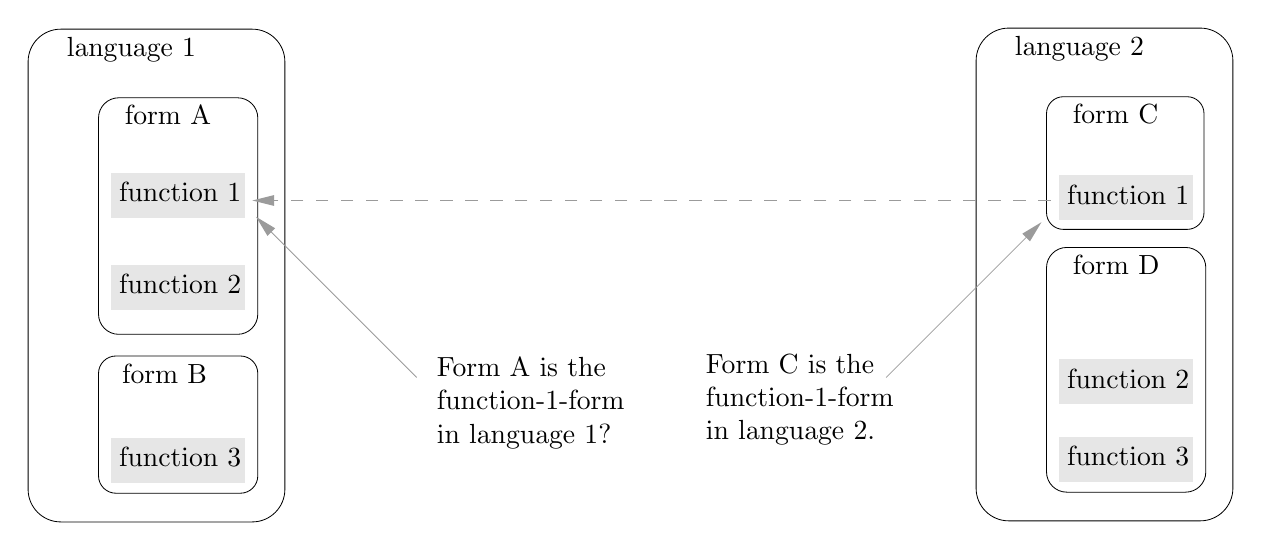
\begin{tikzpicture}[x=0.75pt,y=0.75pt,yscale=-0.87,xscale=0.87]
%uncomment if require: \path (0,394); %set diagram left start at 0, and has height of 394

%Rounded Rect [id:dp765605107552563] 
\draw   (108,68.8) .. controls (108,62.61) and (113.02,57.59) .. (119.21,57.59) -- (185,57.59) .. controls (191.19,57.59) and (196.21,62.61) .. (196.21,68.8) -- (196.21,177.38) .. controls (196.21,183.57) and (191.19,188.59) .. (185,188.59) -- (119.21,188.59) .. controls (113.02,188.59) and (108,183.57) .. (108,177.38) -- cycle ;
%Rounded Rect [id:dp3963315857814693] 
\draw   (108,210.25) .. controls (108,204.91) and (112.33,200.59) .. (117.66,200.59) -- (186.55,200.59) .. controls (191.89,200.59) and (196.21,204.91) .. (196.21,210.25) -- (196.21,266.93) .. controls (196.21,272.26) and (191.89,276.59) .. (186.55,276.59) -- (117.66,276.59) .. controls (112.33,276.59) and (108,272.26) .. (108,266.93) -- cycle ;
%Rounded Rect [id:dp6927975660483339] 
\draw   (69,37.66) .. controls (69,27.68) and (77.09,19.59) .. (87.08,19.59) -- (193.14,19.59) .. controls (203.12,19.59) and (211.21,27.68) .. (211.21,37.66) -- (211.21,274.4) .. controls (211.21,284.38) and (203.12,292.48) .. (193.14,292.48) -- (87.08,292.48) .. controls (77.09,292.48) and (69,284.38) .. (69,274.4) -- cycle ;
%Rounded Rect [id:dp42871723401807316] 
\draw   (633,66.34) .. controls (633,61.18) and (637.18,57) .. (642.34,57) -- (710.87,57) .. controls (716.03,57) and (720.21,61.18) .. (720.21,66.34) -- (720.21,121.14) .. controls (720.21,126.3) and (716.03,130.48) .. (710.87,130.48) -- (642.34,130.48) .. controls (637.18,130.48) and (633,126.3) .. (633,121.14) -- cycle ;
%Rounded Rect [id:dp10003217177182089] 
\draw   (633,151.69) .. controls (633,145.5) and (638.02,140.48) .. (644.21,140.48) -- (710,140.48) .. controls (716.19,140.48) and (721.21,145.5) .. (721.21,151.69) -- (721.21,264.79) .. controls (721.21,270.98) and (716.19,276) .. (710,276) -- (644.21,276) .. controls (638.02,276) and (633,270.98) .. (633,264.79) -- cycle ;
%Rounded Rect [id:dp9442048696447489] 
\draw   (594,37.08) .. controls (594,27.09) and (602.09,19) .. (612.08,19) -- (718.14,19) .. controls (728.12,19) and (736.21,27.09) .. (736.21,37.08) -- (736.21,273.81) .. controls (736.21,283.8) and (728.12,291.89) .. (718.14,291.89) -- (612.08,291.89) .. controls (602.09,291.89) and (594,283.8) .. (594,273.81) -- cycle ;
%Straight Lines [id:da3048128167305082] 
\draw [color={rgb, 255:red, 155; green, 155; blue, 155 }  ,draw opacity=1 ] [dash pattern={on 4.5pt off 4.5pt}]  (635.21,114.48) -- (195.21,114.48) ;
\draw [shift={(193.21,114.48)}, rotate = 360] [fill={rgb, 255:red, 155; green, 155; blue, 155 }  ,fill opacity=1 ][line width=0.08]  [draw opacity=0] (12,-3) -- (0,0) -- (12,3) -- cycle    ;
%Straight Lines [id:da30464466494627773] 
\draw [color={rgb, 255:red, 155; green, 155; blue, 155 }  ,draw opacity=1 ]   (544.21,212.48) -- (628.8,127.89) ;
\draw [shift={(630.21,126.48)}, rotate = 135] [fill={rgb, 255:red, 155; green, 155; blue, 155 }  ,fill opacity=1 ][line width=0.08]  [draw opacity=0] (12,-3) -- (0,0) -- (12,3) -- cycle    ;
%Straight Lines [id:da3716681493529823] 
\draw [color={rgb, 255:red, 155; green, 155; blue, 155 }  ,draw opacity=1 ]   (284.21,212.48) -- (196.63,124.89) ;
\draw [shift={(195.21,123.48)}, rotate = 45] [fill={rgb, 255:red, 155; green, 155; blue, 155 }  ,fill opacity=1 ][line width=0.08]  [draw opacity=0] (12,-3) -- (0,0) -- (12,3) -- cycle    ;

% Text Node
\draw  [draw opacity=0][fill={rgb, 255:red, 230; green, 230; blue, 230 }  ,fill opacity=1 ]  (115,99) -- (189,99) -- (189,124) -- (115,124) -- cycle  ;
\draw (118,103) node [anchor=north west][inner sep=0.75pt]   [align=left] {function 1};
% Text Node
\draw  [draw opacity=0][fill={rgb, 255:red, 230; green, 230; blue, 230 }  ,fill opacity=1 ]  (115,150) -- (189,150) -- (189,175) -- (115,175) -- cycle  ;
\draw (118,154) node [anchor=north west][inner sep=0.75pt]   [align=left] {function 2};
% Text Node
\draw  [draw opacity=0][fill={rgb, 255:red, 230; green, 230; blue, 230 }  ,fill opacity=1 ]  (115,246) -- (189,246) -- (189,271) -- (115,271) -- cycle  ;
\draw (118,250) node [anchor=north west][inner sep=0.75pt]   [align=left] {function 3};
% Text Node
\draw (121.21,60.59) node [anchor=north west][inner sep=0.75pt]   [align=left] {form A};
% Text Node
\draw (119.66,203.59) node [anchor=north west][inner sep=0.75pt]   [align=left] {form B};
% Text Node
\draw (89.08,22.59) node [anchor=north west][inner sep=0.75pt]   [align=left] {language 1};
% Text Node
\draw  [draw opacity=0][fill={rgb, 255:red, 230; green, 230; blue, 230 }  ,fill opacity=1 ]  (640,100.41) -- (714,100.41) -- (714,125.41) -- (640,125.41) -- cycle  ;
\draw (643,104.41) node [anchor=north west][inner sep=0.75pt]   [align=left] {function 1};
% Text Node
\draw  [draw opacity=0][fill={rgb, 255:red, 230; green, 230; blue, 230 }  ,fill opacity=1 ]  (640,202.41) -- (714,202.41) -- (714,227.41) -- (640,227.41) -- cycle  ;
\draw (643,206.41) node [anchor=north west][inner sep=0.75pt]   [align=left] {function 2};
% Text Node
\draw  [draw opacity=0][fill={rgb, 255:red, 230; green, 230; blue, 230 }  ,fill opacity=1 ]  (640,245.41) -- (714,245.41) -- (714,270.41) -- (640,270.41) -- cycle  ;
\draw (643,249.41) node [anchor=north west][inner sep=0.75pt]   [align=left] {function 3};
% Text Node
\draw (646.21,60) node [anchor=north west][inner sep=0.75pt]   [align=left] {form C};
% Text Node
\draw (646.21,143.48) node [anchor=north west][inner sep=0.75pt]   [align=left] {form D};
% Text Node
\draw (614.08,22) node [anchor=north west][inner sep=0.75pt]   [align=left] {language 2};
% Text Node
\draw (443,198) node [anchor=north west][inner sep=0.75pt]   [align=left] {Form C is the \\function-1-form\\in language 2.};
% Text Node
\draw (294,200) node [anchor=north west][inner sep=0.75pt]   [align=left] {Form A is the \\function-1-form\\in language 1?};


\end{tikzpicture}
